\subsection*{Solution to Spring 2015, \# 1}\label{s151}
We mirror the derivation of the Rankine-Hugoniot conditions given in Section 3.4 of Evans.

First assume $v: \R \times [0, \infty) \rightarrow \R$ is smooth with compact support. Then if we pretend
$u$ is a smooth solution to the given conservation law. Since $v$ is of compact support, integration by parts yields
\begin{align*}
0 &= \int_{0}^{\infty}\int_{-\infty}^{\infty}(u_{t} + f(u)_{x} + u)v\, dx\, dt\\
 &= \int_{-\infty}^{\infty}\bigg(-\int_{0}^{\infty}uv_{t}\, dt - uv|_{t = 0}\bigg)\, dx + \int_{0}^{\infty}\bigg(-\int_{-\infty}^{\infty}f(u)v_{x}\, dx\bigg)\, dt + \int_{0}^{\infty}\int_{-\infty}^{\infty}uv\, dx\, dt\\
 &= -\int_{0}^{\infty}\int_{-\infty}^{\infty}uv_{t} + f(u)v_{x} - uv\, dx\, dt - \int_{-\infty}^{\infty}u^{0}(x)v(x, 0)\, dx.
\end{align*}
Thus we define the notion of an integral solution as follows: We say that $u \in L^{\infty}(\R \times (0, \infty))$ is an integral solution
if
\begin{align}\label{s15ran}
-\int_{0}^{\infty}\int_{-\infty}^{\infty}uv_{t} + f(u)v_{x} - uv\, dx\, dt - \int_{-\infty}^{\infty}u^{0}(x)v(x, 0)\, dx = 0
\end{align}
for all smooth $v: \R \times [0, \infty) \rightarrow \R$ with compact support.

Let $V$ be an open region contained in $\R \times (0, \infty)$. Let $V_{\ell}$ be the part of $V$ on the left of a smooth curve $C$
and $V_{r}$ be the part on the right. We assume that $u$ is an integral solution of $u_{t} + f(u)_{x} = -u$ (and so satisfies \eqref{s15ran}) and that
$u$ and its first derivatives are uniformly continuous in $V_{\ell}$ and $V_{r}$.

First, let $\wt{v}$ be a smooth function with compact support in $V_{\ell}$. Then by \eqref{s15ran} since $\wt{v}$ is compactly supported in $V_{\ell} \subset V$,
\begin{align*}
0 = \int_{0}^{\infty}\int_{-\infty}^{\infty}u\wt{v}_{t} + f(u)\wt{v}_{x} - u\wt{v}\, dx\, dt = -\int_{0}^{\infty}\int_{-\infty}^{\infty}(u_{t} + f(u)_{x} + u)\wt{v}\, dx\, dt.
\end{align*}
Therefore since the above equation is true for all smooth $\wt{v}$ with compact support in $V_{\ell}$, we have
$u_{t} + f(u)_{x} + u = 0$ in $V_{\ell}$. Similarly, $u_{t} + f(u)_{x} + u = 0$ in $V_{r}$
(the purpose of this paragraph is to show that if $u$ is an integral solution and is sufficiently smooth,
$u_{t} + f(u)_{x} + u = 0$ in $V_{\ell}$ and $V_{r}$).

Now choose a smooth compactly supported function $v$ with compact support in $V \subset \R \times (0, \infty)$, not necessarily vanishing along
the curve $C$. Again by \eqref{s15ran},
\begin{equation}
\begin{aligned}\label{s15sumint}
0 &= \int_{0}^{\infty}\int_{-\infty}^{\infty}uv_{t} + f(u)v_{x} - uv\, dx\, dt\\
& = \iint_{V_{\ell}}uv_{t} + f(u)v_{x} - uv\, dx\, dt + \iint_{V_{r}}uv_{t} + f(u)v_{x} - uv\, dx\, dt.
\end{aligned}
\end{equation}
Since $v$ has compact support in $V$, integration by parts yields
\begin{equation}
\begin{aligned}\label{s15intleft}
\iint_{V_{\ell}}&uv_{t} + f(u)v_{x} - uv\, dx\, dt\\
 &= -\iint_{V_{\ell}}(u_{t} + f(u)_{x} + u)v\, dx\, dt + \int_{C}(u_{\ell}\nu^{2} + f(u_{\ell})\nu^{1})v\, dl\\
&= \int_{C}(u_{\ell}\nu^{2} + f(u_{\ell})\nu^{1})v\, dl
\end{aligned}
\end{equation}
since $u_{t} + f(u)_{x} + u = 0$ in $V_{\ell}$ where $\nu = (\nu^{1}, \nu^{2})$ is the unit normal to the curve $C$, pointing from $V_{\ell}$ into $V_{r}$
and the subscript $\ell$ denotes the limit from the left. Similarly we have
\begin{align}\label{s15intright}
\iint_{V_{r}}uv_{t} + f(u)v_{x} - uv\, dx\, dt = -\int_{C}(u_{r}\nu^{2} + f(u_{r})\nu^{1})v\, dl.
\end{align}
Adding \eqref{s15intleft} and \eqref{s15intright} and using \eqref{s15sumint}, we have
\begin{align*}
0 = \int_{C}((u_{\ell} - u_{r})\nu^{2} + (f(u_{\ell}) - f(u_{r}))\nu^{1})v\, dl
\end{align*}
for all smooth functions $v$ with compact support in $V$. Therefore
along $C$,
$$(f(u_{r}) - f(u_{\ell}))\nu^{1} + (u_{r} - u_{\ell})\nu^{2} = 0.$$
If we represent $C$ parametrically as $\{(x, t): x = s(t)\}$, then $\nu = (1 + \dot{s}^{2})^{1/2}(1, -\dot{s})$
and hence
$$f(u_{r}) - f(u_{\ell}) = \dot{s}(u_{r} - u_{\ell})$$
along the curve $C$. In the notation of the problem statement, this is
$$f(u_{+}) - f(u_{-}) = \dot{s}(u_{+} - u_{-}).$$
This gives the Rankine-Hugoniot condition along the shock curve $C$.
\hfill\qed

\subsection*{Solution to Spring 2015, \#2}\label{s152}
We will assume that $c$ is differentiable. (Alternatively, the same proof works if we had $\abn{c'(x)} \leq \wh{c}$
instead of $\abn{c(x)} \leq \wh{c}$, because the latter assumption is not really used anywhere.) Let $u, v$ be two compactly
supported smooth solutions to the given PDE. Let $w := u - v$. Then
\begin{align*}
w_{tt} - c(x)^{2}w_{xx} + w_{t} &= 0\quad (x, t) \in \R \times [0, \infty)\\
w(x, 0) &= 0\quad x \in \R\\
w_{t}(x, 0) &= 0\quad x \in \R.
\end{align*}
We mimic the wave energy. Let $$e(t) := \frac{1}{2}\int_{\R}w_{t}^{2} + c(x)^{2}w_{x}^{2}\, dx.$$ Note $e(0) = 0$. We have
\begin{align*}
\dot{e}(t) &= \int_{\R}w_{t}w_{tt} + c(x)^{2}w_{x}w_{xt}\, dx\\
& = \int_{\R}w_{t}w_{tt} - c(x)^{2}w_{xx}w_{t} - 2c(x)c'(x)w_{x}w_{t}\, dx\\
& = \int_{\R}-w_{t}^{2} - 2c(x)c'(x)w_{x}w_{t}\, dx\\
& \leq \int_{\R}-2c'(x)(c(x)w_{x})w_{t}\, dx\\
& \leq 2\|c'\|_{L^{\infty}(\supp w)}\int_{\R}|c(x)w_{x}||w_{t}|\, dx.
\end{align*}
Let $M := 2\|c'\|_{L^{\infty}(\supp w)}$. Then since $ab \leq (a^{2} + b^{2})/2$ for $a, b \geq 0$, it follows that
\begin{align*}
\dot{e}(t) \leq M \cdot \frac{1}{2}\int_{\R}c(x)^{2}w_{x}^{2} + w_{t}^{2}\, dx = Me(t).
\end{align*}
By Gronwall's inequality,
$e(t) \leq e(0)\exp(Mt) = 0$ where the last equality is because $e(0) = 0$. Thus $w_{t} \equiv 0$ and $w_{x} \equiv 0$ which implies $w \equiv 0$ since $w(x, 0) = 0$ for $x \in \R$.
Therefore the PDE has at most one smooth compactly supported solution.
\hfill\qed

\subsection*{Solution to Spring 2015, \#3}\label{s153}
We first solve
\begin{align*}
u_{t} + u_{x}u &= -u\\
u(x, 0) &= x
\end{align*}
as a guide of what we should do in the multidimensional case. In this case we have
\begin{align*}
\begin{array}{ll}
\dot{t}(s) = 1 \quad &t(0) = 0\\
\dot{x}(s) = z \quad &x(0) = x_{0}\\
\dot{z}(s) = -z \quad &z(0) = x_{0}.
\end{array}
\end{align*}
Therefore $t(s) = s$, $z(s) = x_{0}e^{-s}$, and $x(s) = 2x_{0} - x_{0}e^{-s}$.
Thus $x = x_{0}(2 - e^{-t})$ and hence
$$u(x, t) = x_{0}e^{-t} = \frac{e^{-t}x}{2 - e^{-t}} = \frac{x}{2e^{t} - 1}.$$

We now return to the main problem and mimic this argument. We observe that the system can be written as
\begin{align*}
\begin{pmatrix}
u_{1}\\u_{2}
\end{pmatrix}_{t} +
\begin{pmatrix}
(u_{1})_{x_{1}} & (u_{1})_{x_{2}}\\
(u_{2})_{x_{1}} & (u_{2})_{x_{2}}
\end{pmatrix}
\begin{pmatrix}
u_{1}\\ u_{2}
\end{pmatrix} =
-\begin{pmatrix}
u_{1}\\u_{2}
\end{pmatrix}.
\end{align*}
The matrix in the above equation is the Jacobian of $\mathbf{u} = (\begin{smallmatrix}u_{1}\\u_{2}\end{smallmatrix})$ and so is the higher dimensional
analogue of $u_{x}$. We once again have
\begin{align*}
\begin{array}{ll}
\dot{t}(s) = 1 \quad & t(0) = 0\\
\dot{\mathbf{x}}(s) = \mathbf{z} \quad & \mathbf{x}(0) = \mathbf{x_{0}} = \begin{pmatrix}x_{0}^{1}\\x_{0}^{2}\end{pmatrix}\\
\dot{\mathbf{z}}(s) = -\operatorname{Id} \mathbf{z} \quad & \mathbf{z}(0) = \begin{pmatrix}-x_{0}^{2}\\x_{0}^{1}\end{pmatrix}.
\end{array}
\end{align*}
Therefore $t(s) = s$ and
$$\mathbf{z}(s) = \begin{pmatrix} -x_{0}^{2}e^{-s}\\x_{0}^{1}e^{-s}\end{pmatrix}.$$
To find $\mb{x}$, we want to solve $\dot{x_{1}}(s) = -x_{0}^{2}e^{-s}$ and $\dot{x_{2}}(s) = x_{0}^{1}e^{-s}$ and hence combining this with the initial conditions
gives
\begin{align*}
\mb{x}(s) = \pmat{1}{-1}{1}{1}\vct{x_{0}^{1}}{x_{0}^{2}} + \vct{x_{0}^{2}}{-x_{0}^{1}}e^{-s} = \left(\pmat{1}{-1}{1}{1} + \pmat{0}{1}{-1}{0}e^{-s}\right)\vct{x_{0}^{1}}{x_{0}^{2}}
\end{align*}
Therefore
\begin{align*}
\mb{u}(\mb{x}, t) &= \pmat{0}{-1}{1}{0}\vct{x_{0}^{1}}{x_{0}^{2}}e^{-s}\\
& = \pmat{0}{-1}{1}{0}\left(\pmat{1}{-1}{1}{1} + \pmat{0}{1}{-1}{0}e^{-t}\right)^{-1}\vct{x_{1}}{x_{2}}e^{-t}\\
& = \frac{1}{2e^{t} - 2 + e^{-t}}\pmat{1 - e^{-t}}{-1}{1}{1 - e^{-t}}\vct{x_{1}}{x_{2}}.
\end{align*}
\hfill\qed

\subsection*{Solution to Spring 2015, \#4}\label{s154}

\subsubsection*{Solution to $4a$}
Let $u = u_{\ell}1_{(0, 1/2)} + u_{r}1_{(1/2, 1)}$. Then the total variation of $u$ is given by
the supremum of $\int_{0}^{1}u(x)\phi'(x)\, dx$ for differentiable $\phi$ vanishing at both 0 and 1 and $\abn{\phi} \leq 1$.
As
\begin{align*}
\int_{0}^{1}u(x)\phi'(x)\, dx = u_{\ell}\int_{0}^{1/2}\phi'(x)\, dx + u_{r}\int_{1/2}^{1}\phi'(x)\, dx = (u_{\ell} - u_{r})\phi(1/2),
\end{align*}
by the arbitrariness of $\phi$, we have that the total variation of $u$ is given by $\abn{u_{\ell} - u_{r}}$ (with the worse case occurring
when $\phi(1/2) = \pm 1$). Thus in this case,
\begin{align*}
E[u] = \frac{1}{8}\abn{u_{\ell} - u_{r}} + \int_{0}^{1/2}\abn{u_{\ell}}^{2}\, dx + \int_{1/2}^{1} \abn{u_{r} - 1}^{2}\, dx = \frac{1}{8}\abn{u_{\ell} - u_{r}} + \frac{1}{2}u_{\ell}^{2} + \frac{1}{2}(u_{r} - 1)^{2}.
\end{align*}
Thus we wish to minimize
$$f(x, y) := \frac{1}{8}\abn{x - y} + \frac{1}{2}x^{2} + \frac{1}{2}(y - 1)^{2}.$$
We compute
\begin{align*}
f_{x}(x, y) =
\begin{cases}
1/8 + x & \text{ if } x > y\\
-1/8 + x & \text{ if } x < y
\end{cases}
\end{align*}
and
\begin{align*}
f_{y}(x, y) =
\begin{cases}
-9/8 + y & \text{ if } x > y\\
-7/8 + y & \text{ if } x < y.
\end{cases}
\end{align*}
Therefore the critical points for $f(x, y)$ are when $x = y$ (since the derivative does not exist at these points)
and $(1/8, 7/8)$ (note that $(-1/8, 9/8)$ is not a critical point since we have the extra condition that $x > y$ and $-1/8 \not> 9/8$).
Since $f(1/8, 7/8) = 7/64$ and $f(x, x) = x^{2} - x + 1 \geq 3/4$ for all $x$, the piecewise constant function with minimal energy is
$$u = \frac{1}{8}1_{(0, 1/2)} + \frac{7}{8}1_{(1/2, 1)}$$
with $E[u] = 7/64$.
\hfill\qed

\subsubsection*{Solution to $4b$}
We now show that there is no $C^{1}$ function $u$ with energy lower than $7/64$.

Let $u$ be a continuous and almost everywhere differentiable function with minimal energy (we will assume such a minimizer exists).
We avoid working directly with $C^{1}$ functions here to avoid technicalities later (namely, if $u \in C^{1}$, $\max(u, 1)$ is not necessarily in $C^{1}$).
We claim that $u \leq 1$ for every $x$. Let $v(x) := \min(u(x), 1)$. We claim that $E[v] \leq E[u]$. We have
\begin{align*}
E[v] &= \frac{1}{8}\int_{\{u \leq 1\}\cap (0, 1)}|u'|\, dx + \int_{0}^{1}|v - g|^{2}\, dx\\
& = \frac{1}{8}\int_{\{u \leq 1\} \cap (0, 1)}|u'|\, dx + \int_{\{u \leq 1\} \cap (0, 1)}|u - g|^{2}\, dx + \int_{\{u > 1\} \cap (0, 1/2)}1\, dx\\
&\leq \frac{1}{8}\int_{0}^{1}|u'|\, dx + \int_{\{u \leq 1\} \cap (0, 1)}|u - g|^{2}\, dx + \int_{\{u > 1\} \cap (0, 1)}|u - g|^{2}\, dx = E[u]
\end{align*}
where the first inequality is because
\begin{align*}
\int_{\{u > 1\} \cap (0, 1)}|u - g|^{2}\, dx &= \int_{\{u > 1\} \cap (0, 1/2)}|u|^{2}\, dx + \int_{\{u > 1\} \cap (1/2, 1)}|u - 1|^{2}\, dx\\
& \geq \int_{\{u > 1\} \cap (0, 1/2)}1\, dx + \int_{\{u > 1\} \cap (1/2, 1)}|u - 1|^{2}\, dx \geq \int_{\{u > 1\} \cap (0, 1/2)}1\, dx.
\end{align*}
Since $u$ has the smallest energy, we must have $u \leq v$ and hence $u = v = \min(u(x), 1)$ which implies
that $u \leq 1$ everywhere.

Next we claim that $u \geq 0$ for every $x$. Let $w(x) := \max(u(x), 0)$. We claim that $E[w] \leq E[u]$. We have
\begin{align*}
E[w] &= \frac{1}{8}\int_{\{u \geq 0\} \cap (0, 1)}\abn{u'}\, dx + \int_{0}^{1}|w - g|^{2}\, dx\\
&= \frac{1}{8}\int_{\{u \geq 0\} \cap (0, 1)}\abn{u'}\, dx + \int_{\{u \geq 0\} \cap (0, 1)}|u - g|^{2}\, dx + \int_{\{u < 0\} \cap (1/2, 1)}1\, dx\\
&\leq \frac{1}{8}\int_{0}^{1}\abn{u'}\, dx + \int_{\{u \geq 0\} \cap (0, 1)}|u - g|^{2}\, dx + \int_{\{u < 0\} \cap (0, 1)}|u - g|^{2}\, dx = E[u]
\end{align*}
where the first inequality is because
\begin{align*}
\int_{\{u < 0\} \cap (0, 1)}|u - g|^{2}\, dx &= \int_{\{u < 0\} \cap (0, 1/2)}|u|^{2}\, dx + \int_{\{u < 0\} \cap (1/2, 1)}|u - 1|^{2}\, dx\\
&\geq  \int_{\{u < 0\} \cap (0, 1/2)}|u|^{2}\, dx + \int_{\{u < 0\} \cap (1/2, 1)}1\, dx \geq \int_{\{u < 0\} \cap (1/2, 1)}1\, dx.
\end{align*}
Since $u$ has the smallest energy, we must have $u \leq w$ and hence $u = w = \max(u(x) , 0)$ and hence $u \geq 0$ everywhere.

Next we claim that $1 - u(1 -x)$ has the same energy as $u$. Indeed,
\begin{align*}
E[1 - u(1 - x)] &= \frac{1}{8}\int_{0}^{1}|u'(x)|\, dx + \int_{0}^{1}|1 - u(1 - x) - g(x)|^{2}\, dx\\
& = \frac{1}{8}\int_{0}^{1}|u'(x)|\, dx + \int_{0}^{1/2}(1 - u(1 - x))^{2}\, dx + \int_{1/2}^{1}(u(1 - x))^{2}\, dx = E[u]
\end{align*}
where the last equality is by the change of variables $x \mapsto 1 - x$.

Finally, we claim that $u(x) = 1 - u(1 - x)$. Since $E[\,\cdot\,]$ is convex,
\begin{align*}
E[\frac{1 - u(1 - x)}{2} + \frac{u(x)}{2}] \leq \frac{1}{2}E[1 - u(1- x)] + \frac{1}{2}E[u] = E[u].
\end{align*}
Therefore since $u$ has minimal energy, we must have
$$\frac{1 - u(1 - x)}{2} + \frac{u(x)}{2} = u(x),$$
that is, $u(x) = 1 - u(1 - x)$.
Thus we have shown that any minimizer $u$ must satisfy $0 \leq u \leq 1$ and $u(x) = 1 - u(1 - x)$.

Let $m := \min_{x \in [0, 1]}u(x) = u(a)$ and $M := \max_{x \in [0, 1]}u(x) = u(b)$.
Note that
$$M = u(b) = 1 - u(1 - b) \leq 1 - m$$
and
$$1 - m = 1 - u(a) = u(1 - a) \leq M$$
which implies that $M = 1 - m$. Since
$$0 \leq m \leq M = 1 -m \leq 1,$$ we must have $m \in [0, 1/2]$.
Let $I$ denote the interval with endpoints $a$ and $b$. We have
\begin{align*}
\int_{0}^{1}|u'(x)|\, dx \geq \int_{I}|u'(x)|\, dx  \geq \bigg|\int_{I}u'(x)\, dx\bigg| \geq |u(b) - u(a)| = M - m = 1 - 2m
\end{align*}
and
\begin{align*}
\int_{0}^{1}|u(x) - g(x)|^{2}\, dx &= \int_{0}^{1/2}|u(x)|^{2}\, dx + \int_{1/2}^{1}|u(x) - 1|^{2}\, dx\\
& \geq \frac{1}{2}m^{2} + \int_{1/2}^{1}(1 - u(x))^{2}\, dx \geq \frac{1}{2}m^{2} + \frac{1}{2}(1 - M)^{2} = m^{2}
\end{align*}
where in the second inequality we have used that $u \leq 1$.
Therefore
$$E[u] \geq \frac{1}{8}(1 - 2m) + m^{2}$$
with $m\in [0, 1/2]$. Minimizing $(1/8)(1 - 2m) + m^{2}$ over $[0, 1/2]$, we see that $$E[u] \geq \frac{1}{8}(1 - \frac{1}{4}) + \frac{1}{64} = \frac{7}{64}$$
and this occurs when $m = 1/8$. Therefore any continuous energy minimizer $u$ which is also almost everywhere differentiable must have a minimum of $1/8$ and a maximum of $7/8$ and
has energy $\geq 7/64$.

We now construct infinitely many continuous and almost everywhere differentiable functions $u_{n}$ such that $E[u_n]$ is arbitrarily close to $7/64$.
Let
\begin{align*}
u_{n}(x) =
\begin{cases}
1/8 & \text{ if } 0 < x < \frac{1}{2} - \frac{1}{n}\\
L_{n}(x) & \text{ if } \frac{1}{2} - \frac{1}{n} \leq x \leq \frac{1}{2} + \frac{1}{n}\\
7/8 & \text{ if } \frac{1}{2} + \frac{1}{n} < x < 1
\end{cases}
\end{align*}
where $L_n(x)$ is the line created by connecting the points $(\frac{1}{2} - \frac{1}{n}, \frac{1}{8})$
and $(\frac{1}{2} + \frac{1}{n}, \frac{7}{8})$.
Therefore
$$L_{n}(x) = \frac{3n}{8}(x - \frac{1}{2} - \frac{1}{n}) + \frac{7}{8}.$$
Then $u_{n}$ is a continuous and almost everywhere differentiable function.
We compute
\begin{align*}
E[u_{n}] &= \frac{1}{8}\int_{1/2 - 1/n}^{1/2 + 1/n}|L_{n}'|\, dx + \int_{0}^{1/2}|u_{n}|^{2} + \int_{1/2}^{1}|u_{n} - 1|^{2}\, dx\\
&= \frac{6}{64} + \bigg(\frac{1}{2} - \frac{1}{n}\bigg)\frac{1}{64} + \int_{1/2 - 1/n}^{1/2}\bigg(\frac{3n}{8}(x - \frac{1}{2} - \frac{1}{n}) + \frac{7}{8}\bigg)^{2}\, dx\\
&\hspace{1.5in} + \int_{1/2}^{1/2 + 1/n}\bigg(\frac{3n}{8}(x - \frac{1}{2} - \frac{1}{n}) - \frac{1}{8}\bigg)^{2}\, dx + \bigg(\frac{1}{2} - \frac{1}{n}\bigg)\frac{1}{64}\\
&= \frac{6}{64} + \bigg(\frac{1}{2} - \frac{1}{n}\bigg)\frac{1}{64} + \frac{7}{64n} + \frac{7}{64n} + \bigg(\frac{1}{2} - \frac{1}{n}\bigg)\frac{1}{64}\\
& = \frac{7}{64} + \frac{3}{16n}.
\end{align*}

Now suppose there was a $C^{1}$ function $\wt{u}$ with minimal energy. If $E[\wt{u}] > 7/64$, then there exists an $N$ sufficiently large (depending on $\wt{u}$) such that $E[\wt{u}] > E[u_{N}]$,
contradicting minimality of $\wt{u}$. Therefore $E[\wt{u}] \leq 7/64$. But by the above discussion, $\wt{u}$ must have a minimum of $1/8$, a maximum of $7/8$, and
have energy $\geq 7/64$. Therefore $E[\wt{u}] = 7/64$. Thus there is no $C^{1}$ function with energy lower than the optimal piecewise constant function
in part $(a)$.
\hfill\qed

%\subsection*{Solution to Spring 2015, \#5}\label{s155}
%Let $w(x, t) := u(x, t) - v(x, t) - \vep e^{2mt}$. Note that $w(x, 0) < 0$. We claim that $w(x, t) < 0$ for all $t > 0$.
%Suppose not. Then there exists a minimal time $t_{0}$ and a corresponding $x_{0}$ such that $w(x_{0}, t_{0}) = 0$ (as $w(x, 0) < 0$, $w$ is continuous
%and $t_{0}$ is minimal). Since $w(x, t_{0}) \leq 0$ for all $x$, $x_{0}$ is a local maximum for $w(x, t_{0})$ as a function of $x$
%and hence $(\Delta w)(x_{0}, t_{0}) \leq 0$. Since $w(x, t') < 0$ for all $(x, t')$ with $t' < t_{0}$, $w_{t}(x_{0}, t_{0}) \geq 0$. Therefore at $(x_{0}, t_{0})$,
%\begin{align}\label{s155eq1}
%w_{t} - \Delta w \geq 0.
%\end{align}
%However, we compute
%\begin{align*}
%w_{t} - \Delta w = u_{t} - v_{t} - 2M\vep e^{2Mt} - \Delta u + \Delta v = -u^{2} + v^{2} - 2M\vep e^{2Mt}.
%\end{align*}
%Since $w(x_{0}, t_{0}) = 0$, $u(x_{0}, t_{0}) = v(x_{0}, t_{0}) + \vep e^{2Mt_{0}}$. Thus at $(x_{0}, t_{0})$,
%\begin{align*}
%w_{t} - \Delta w &= -(v(x_0, t_0) + \vep e^{2Mt_{0}})^{2} + v(x_{0}, t_{0})^{2} - 2M\vep e^{2Mt_{0}}\\
%& = -2\vep v(x_{0}, t_{0})e^{2Mt_{0}} - \vep^{2}e^{4Mt_{0}} - 2M\vep e^{2Mt_{0}}\\
%& = \vep e^{2Mt_{0}}(-2M - 2v(x_{0}, t_{0}) - \vep e^{2Mt_{0}}) < 0
%\end{align*}
%since $|v(x_{0}, t_{0})| \leq M$. This contradicts \eqref{s155eq1} and hence $w(x, t) < 0$ for all $t > 0$. That is,
%$$u(x, t) < v(x, t) + \vep e^{2Mt}.$$
%Interchanging the role of $u$ and $v$ (and using that $|u| \leq M$) yields that $v(x, t) < u(x, t) + \vep e^{2Mt}$.
%Thus $$\abn{u(x, t) - v(x, t)} < \vep e^{2Mt}.$$
\subsection*{Solution to Spring 2015, \#5}\label{s155}
Define $w(x,t) := u(x,t) - v(x,t) - \epsilon e^{2Mt}$, where $\epsilon$ is from the condition $ |u(x,0) - v(x,0)| < \epsilon$ and $M$ is from $|u|, |v| \leq M$. We aim to show that $w < 0$ for all $(x,t)$. First, observe that
$$ w(x,0) = u(x,0) - v(x,0) - \epsilon < 0 $$
By contradiction, suppose there exists $(x_0,t_0)$ such that $w(x_0,t_0) = 0$. Furthermore, let $t_0$ be the first time for which this happens. Now, consider $w(x,t_0)$ as a function of $x$. Because $w(x,t) < 0 $ for all $x \in \R^n$ and $t < t_0$ and $w(x_0,t_0) = 0$ for all $x \in \R^n$, we have that $w(x,t_0) \leq 0$ for all $x \in \R^n$, implying that $x = x_0$ is a local maximum for $w(x,t_0)$. Hence, $\Delta_x w(x_0,t_0) \leq 0$. We also know that $w_t(x_0,t_0) \geq 0$. Thus, it follows that
$$ (w_t - \Delta_x w)(x_0,t_0) \geq 0 $$
However, at the same time
\begin{align*}
	(w_t - \Delta w)(x_0,t_0) &= (u_t - \Delta u)(x_0,t_0) - (v_t - \Delta v)(x_0,t_0) - 2M \epsilon e^{2M t_0} \\
	&= -u^2 (x_0,t_0) + v^2(x_0,t_0) - 2M \epsilon e^{2Mt_0} \\
	&= -(v(x_0,t_0) + \epsilon e^{2Mt_0})^2 + v^2(x_0,t_0) - 2M \epsilon e^{2Mt_0} \\
	&= -2 \epsilon v(x_0,t_0) e^{2Mt_0} - \epsilon^2 e^{4Mt_0} - 2M \epsilon e^{2Mt_0} \\
	&\leq -\epsilon^2 e^{4Mt_0} \\
	&< 0
\end{align*}
where the third equality is because $w(x_0,t_0) = 0$ and the second-to-last inequality is because $|v| \leq M$. Hence, we have reached a contradiction. Therefore, there does not exist a point $(x_0,t_0)$ such that $w(x_0,t_0) = 0$, and because $w$ is continuous in both variables, we have
$$ w(x,t) < 0 \quad \implies \quad u(x,t) - v(x,t) < \epsilon e^{2Mt} $$
for all $x \in \R^n$ and $t > 0$. If we were to repeat the argument above but with the roles of $u$ and $v$ swapped, meaning we consider the function $y(x,t) := v(x,t) - u(x,t) - \epsilon e^{2Mt}$, we will reach the conclusion
$$ y(x,t) < 0 \quad \implies \quad v(x,t) - u(x,t) < \epsilon e^{2Mt} $$
for all $x \in \R^n$ and $t >0$. Therefore, we have
$$ |u(x,t) - v(x,t)| < \epsilon e^{2Mt} $$
for all $x$ and $t$.
\hfill\qed

\subsection*{Solution to Spring 2015, \#6}\label{s156}
We will denote the Green's function by $G(x, \xi)$ and by $G'(x, \xi)$, we mean $\frac{d}{dx}G(x, \xi)$.
\subsubsection*{Solution to $6a$}
We solve
\begin{align}\label{s156aeq1}
\frac{d^{2}}{dx^{2}}G(x, \xi) - \frac{6}{x^{2}}G(x, \xi) = \delta(x - \xi)
\end{align}
where $G(0, \xi) = 0$ and $G(x, \xi) \rightarrow 0$ as $x \rightarrow \infty$.
The homogenous solutions to $y'' - 6y/x^{2} = 0$ are $x^{3}$ and $x^{-2}$. Therefore
\begin{align*}
G(x, \xi) =
\begin{cases}
ax^{-2} + bx^{3} & \text{ if } x < \xi\\
cx^{-2} + dx^{3} & \text{ if } x > \xi.
\end{cases}
\end{align*}
Since $G(0, \xi) = 0$ and $G(\infty, 0) = 0$, $a = 0$ and $d = 0$.
We also want $G$ to be continuous when $x = \xi$. So we want
$$b \xi^{3} = c\xi^{-2}$$
and hence $c = b\xi^{5}$. If we integrate \eqref{s156aeq1}, then
\begin{align*}
\int_{\xi^{-}}^{\xi^{+}}\frac{d^{2}}{dx^{2}}G(x, \xi)\, dx - \int_{\xi^{-}}^{\xi^{+}}\frac{6}{x^{2}}G(x, \xi)\, dx = \int_{\xi^{-}}{\xi^{+}}\delta(x - \xi)\, dx
\end{align*}
and hence as $G$ is continuous, it follows that $G'(\xi^{+}, \xi) - G'(\xi^{-}, \xi) = 1$. We have
\begin{align*}
G(x, \xi) =
\begin{cases}
bx^{3} & \text{ if } x < \xi\\
b\xi^{5}x^{-2} & \text{ if } x > \xi.
\end{cases}
\end{align*}
Then
\begin{align*}
G'(x, \xi) =
\begin{cases}
3bx^{2} & \text{ if } x < \xi\\
-2b\xi^{5}x^{-3} & \text{ if } x > \xi
\end{cases}
\end{align*}
and hence
\begin{align*}
1 = G'(\xi^{+}, \xi) - G'(\xi^{-}, \xi) = -2b\xi^{2} - 3b\xi^{2} = -5b\xi^{2}.
\end{align*}
Therefore $b = -1/(5\xi^{2})$ and hence
\begin{align*}
G(x, \xi) =
\begin{cases}
-x^{3}/(5\xi^{2}) & \text{ if } x < \xi\\
-\xi^{3}/(5x^{2}) & \text{ if } x > \xi.
\end{cases}
\end{align*}
\hfill\qed

\subsubsection*{Solution to $6b$}
\begin{enumerate}
\item[$(i)$] Since $f$ has a jump discontinuity at $x = 1$, the appropriate continuity conditions for $y$ at $x = 1$ is
\begin{enumerate}
\item $y$ is differentiable at $x = 1$
\item $y'$ is continuous at $x = 1$
\item $y''$ has a jump discontinuity at $x = 1$.
\end{enumerate}
\item[$(ii)$] We have
\begin{align*}
y(x) = \int_{0}^{\infty}G(x, \xi)f(\xi)\, d\xi = \int_{0}^{1}-\frac{x^{3}}{5\xi^{2}}1_{x < \xi} - \frac{\xi^{3}}{5x^{2}}1_{x > \xi}\, d\xi.
\end{align*}
If $x \geq 1$, then
\begin{align*}
 \int_{0}^{1}-\frac{x^{3}}{5\xi^{2}}1_{x < \xi} - \frac{\xi^{3}}{5x^{2}}1_{x > \xi}\, d\xi = -\frac{1}{5x^{2}}\int_{0}^{1}\xi^{3}\, d\xi = -\frac{1}{20x^{2}}.
\end{align*}
If $x < 1$, then
\begin{align*}
 \int_{0}^{1}-\frac{x^{3}}{5\xi^{2}}1_{x < \xi} - \frac{\xi^{3}}{5x^{2}}1_{x > \xi}\, d\xi & = \int_{x}^{1}-\frac{x^{3}}{5\xi^{2}}\, d\xi + \int_{0}^{x}-\frac{\xi^{3}}{5x^{2}}\, d\xi\\
 & = -\frac{x^{3}}{5}\int_{x}^{1}\frac{1}{\xi^{2}}\, d\xi - \frac{1}{5x^{2}}\int_{0}^{x}\xi^{2}\, d\xi = \frac{1}{5}x^{3} - \frac{1}{4}x^{2}.
\end{align*}
Therefore
$$y(x) = \bigg(\frac{1}{5}x^{3} - \frac{1}{4}x^{2}\bigg)1_{x < 1} - \frac{1}{20x^{2}}1_{x \geq 1}.$$
\end{enumerate}
\hfill\qed

\subsection*{Solution to Spring 2015, \#7}\label{s157}
We will assume that $$h(x, t) = a(t)\psi(x/\ell(t))$$ and let $\eta := x/\ell(t)$. Note that in what follows $\psi'(\eta) = d\psi/d\eta$.
Then
\begin{align*}
h_{t} &= a'(t)\psi(\eta) + a(t)\psi'(\eta)x(-\ell(t)^{-2})\ell'(t)\\
& = a'(t)\psi(\eta) - a(t)\psi'(\eta)x\frac{\ell'(t)}{\ell(t)^{2}} = a'(t)\psi(\eta) - a(t)\psi'(\eta)\eta\frac{\ell'(t)}{\ell(t)}.
\end{align*}
Since
$$h_{x} = \frac{a(t)}{\ell(t)}\psi'(\eta) \quad \text{ and } \quad h^{3} = a(t)^{3}\psi(\eta)^{3}$$
it follows that
\begin{align*}
(h^{3}h_{x})_{x} &= \frac{a(t)^{4}}{\ell(t)}(\psi(\eta)^{3}\psi'(\eta))_{x} = \frac{a(t)^{4}}{\ell(t)}(3\psi(\eta)^{2}\psi'(\eta)^{2}\frac{1}{\ell(t)} + \psi(\eta)^{3}\psi''(\eta)\frac{1}{\ell(t)})\\
&=\frac{a(t)^{4}}{\ell(t)^{2}}(3\psi(\eta)^{2}\psi'(\eta)^{2} + \psi(\eta)^{3}\psi''(\eta))
\end{align*}
and hence
\begin{align*}
\frac{1}{3}(h^{3}h_{x})_{x} = \frac{a(t)^{4}}{\ell(t)^{2}}(\psi(\eta)^{2}\psi'(\eta)^{2} + \frac{1}{3}\psi(\eta)^{3}\psi''(\eta)).
\end{align*}
Since $h_{t} = \frac{1}{3}(h^{3}h_{x})_{x}$, we have
\begin{align}\label{s157eq1}
\frac{\ell(t)^{2}}{a(t)^{4}}\bigg(a'(t)\psi(\eta) - a(t)\psi'(\eta)\eta\frac{\ell'(t)}{\ell(t)}\bigg) = \psi(\eta)^{2}\psi'(\eta)^{2} + \frac{1}{3}\psi(\eta)^{3}\psi''(\eta).
\end{align}
Let $a(t) := t^{\alpha}$ and $\ell(t) := t^{\beta}$. Then
\begin{align*}
\frac{\ell(t)^{2}}{a(t)^{4}}a'(t) = \alpha t^{2\beta - 3\alpha - 1}
\end{align*}
and
\begin{align*}
\frac{\ell(t)^{2}}{a(t)^{4}}a(t)\frac{\ell(t)}{\ell'(t)} = \frac{\ell(t)}{a(t)^{3}}\ell'(t) = \beta t^{2\beta - 3\alpha - 1}.
\end{align*}
Balancing powers of $t$ in \eqref{s157eq1}, we must have
\begin{align}\label{s157eq2}
2\beta - 3\alpha = 1.
\end{align}
With this condition on $\alpha$ and $\beta$, this changes \eqref{s157eq1} into
\begin{align}\label{s157eq3}
\alpha\psi(\eta) - \beta\psi'(\eta)\eta = \psi(\eta)^{2}\psi'(\eta)^{2} + \frac{1}{3}\psi(\eta)^{3}\psi''(\eta).
\end{align}
We now use the boundary conditions to give another relation between $\alpha$ and $\beta$.
We have
\begin{align*}
1 = \int_{-L(t)}^{L(t)}h(x, t)\, dx = \int_{-L(t)}^{L(t)}t^{\alpha}\psi(x/t^{\beta})\, dx = \int_{-L(t)/t^{\beta}}^{L(t)/t^{\beta}}t^{\alpha + \beta}\psi(s)\, ds
\end{align*}
and hence
\begin{align*}
\int_{-L(t)/t^{\beta}}^{L(t)/t^{\beta}}\psi(s)\, ds = t^{-\alpha - \beta}.
\end{align*}
Taking the time derivative of both sides gives
\begin{align*}
\psi(\frac{L(t)}{t^{\beta}})\frac{d}{dt}(\frac{L(t)}{t^{\beta}}) - \psi(-\frac{L(t)}{t^{\beta}})\frac{d}{dt}(-\frac{L(t)}{t^{\beta}}) = (-\alpha - \beta)t^{-\alpha - \beta - 1}.
\end{align*}
Since $h(\pm L(t), t) = 0$,
$$0 = t^{\alpha}\psi(\pm\frac{L(t)}{t^{\beta}})$$
and hence $\psi(\pm L(t)/t^{\beta}) = 0$.
Therefore we must also have
\begin{align}\label{s157eq4}
-\alpha - \beta = 0.
\end{align}
Combining \eqref{s157eq2} and \eqref{s157eq4} gives that
$$\alpha = -1/5 \quad \text{ and } \quad \beta = 1/5.$$
Then \eqref{s157eq3} becomes
\begin{align*}
-\frac{1}{5}\psi(\eta) - \frac{1}{5}\psi'(\eta)\eta &= \psi(\eta)^{2}\psi'(\eta)^{2} + \frac{1}{3}\psi(\eta)^{3}\psi''(\eta)\\
-(\psi(\eta) + \psi'(\eta)\eta) &= 5\psi(\eta)^{2}\psi'(\eta)^{2} + \frac{5}{3}\psi(\eta)^{3}\psi''(\eta)
\end{align*}
and hence
\begin{align*}
-(\eta\psi(\eta))' &= (\frac{5}{3}\psi(\eta)^{3}\psi'(\eta))'.
\end{align*}
Therefore
$$-\eta\psi(\eta) = \frac{5}{3}\psi(\eta)^{3}\psi'(\eta) + C.$$
Take $\eta = L(t)/t^{1/5}$. Then with this choice of $\eta$, $\psi(\eta) = 0$ and hence $C = 0$. Thus
$$-\eta\psi(\eta) = \frac{5}{3}\psi(\eta)^{3}\psi'(\eta).$$
This equation is now separable. Solving yields
\begin{align*}
-\frac{1}{2}\eta^{2} = \frac{5}{9}\psi^{3} + \wt{C}.
\end{align*}
Take $\eta = L(t)/t^{1/5}$, then $$\wt{C} = -\frac{1}{2}\bigg(\frac{L(t)}{t^{1/5}}\bigg)^{2} = -\frac{1}{2}\cdot \frac{L^{2}}{t^{2/5}}.$$
Therefore
$$\frac{5}{9}\psi^{3} = \frac{1}{2}\bigg(\frac{L^{2}}{t^{2/5}} - \eta^{2}\bigg)$$
and hence
$$\psi(\eta) = \bigg(\frac{9}{10}\bigg)^{1/3}\bigg(\frac{L^{2}}{t^{2/5}} - \eta^{2}\bigg)^{1/3}.$$
Since $\eta = x/\ell(t) = x/t^{1/5}$,
\begin{align*}
h(x, t) = t^{-1/5}\bigg(\frac{9}{10}\bigg)^{1/3}\bigg(\frac{L^{2}}{t^{2/5}} - \frac{x^{2}}{t^{2/5}}\bigg)^{1/3} = \bigg(\frac{9}{10}\bigg)^{1/3}t^{-1/3}(L^{2} - x^{2})^{1/3}.
\end{align*}
Now we compute $L(t)$. Since $\int_{-L(t)}^{L(t)}h(x, t)\, dx = 1$,
\begin{align*}
\bigg(\frac{9}{10t}\bigg)^{1/3}\int_{-L}^{L}(L^{2} - x^{2})^{1/3}\, dx = 1.
\end{align*}
Rearranging and making the change of variables $x = L\sin\ta$ yields that
\begin{align*}
\bigg(\frac{10t}{9}\bigg)^{1/3} = L\int_{-\pi/2}^{\pi/2}(\cos^{2/3}\ta)\cos \ta\, d\ta = 2L\int_{0}^{\pi/2}\cos^{5/3}\ta\, d\ta.
\end{align*}
Therefore
$$L(t) = \bigg(\frac{10t}{9}\bigg)^{1/3}\bigg(2\int_{0}^{\pi/2}\cos^{5/3}\ta\, d\ta\bigg)^{-1}$$
and
$$h(x, t) = \bigg(\frac{9}{10t}\bigg)^{1/3}(L^{2} - x^{2})^{1/3}.$$
\hfill\qed

\subsection*{Solution to Spring 2015, \#8}\label{s158}
\subsubsection*{Solution to $8a$}
The equilibrium points are
$$(x, y) = (0, 0), (1, 1), (-1, -1), (1, -1), (-1, 1).$$
The Jacobian is
$$J(x, y) = \pmat{1 - y^{2}}{-2xy}{-2xy}{1 - x^{2}}.$$
The Jacobian at $(0, 0)$ is $\smat{1}{0}{0}{1}$, the Jacobian at $(1, 1)$ and $(-1, -1)$
is $\smat{0}{-2}{-2}{0}$, and the Jacobian at $(1, -1)$ and $(-1, 1)$ is $\smat{0}{2}{2}{0}$.

The eigenvalues of $\smat{1}{0}{0}{1}$ are $1, 1$ and the eigenvectors are $\svt{1}{0}$ and $\svt{0}{1}$.
The eigenvalues of $\smat{0}{-2}{-2}{0}$ are $2, -2$ and the corresponding eigenvectors are $\svt{1}{-1}$ and
$\svt{1}{1}$. The eigenvalues of $\smat{0}{2}{2}{0}$ are $2, -2$ and the corresponding eigenvectors are $\svt{1}{1}$ and $\svt{1}{-1}$.
Therefore $(0, 0)$ is a source node and $(\pm 1, \pm 1)$ are all saddles.
The phase portrait is as follows:

\begin{center}
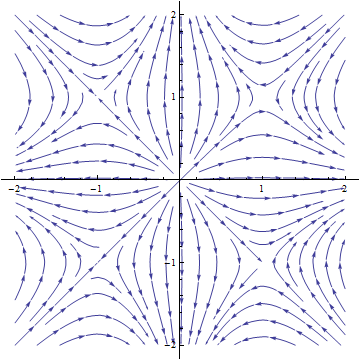
\includegraphics[scale=0.75]{./_Figures/S158.png}
\end{center}

For large $x, y$, $1 - y^{2} \approx -y^{2}$ and $1 - x^{2} \approx -x^{2}$. Then
\begin{align*}
\frac{dy}{dx} \approx \frac{x}{y}
\end{align*}
and hence for large $x$ and large $y$, the trajectories looks like $x^{2} - y^{2} = C$, in other words, the trajectories for large $x$, $y$
are hyperbolas.
\hfill\qed

\subsubsection*{Solution to $8b$}
The Jacobian in this case is
$$J(x, y) = \pmat{1 - y^{2}}{-2xy}{-2xy^{2}}{2y(1 - x^{2})}$$
and so $J(1, -1) = \smat{0}{2}{-2}{0}$ which has eigenvalues $\pm 2i$. Therefore $(1, -1)$ is either a center or spiral.
To prove $(1, -1)$ is stable, we use Lyapunov theory. We solve
$$\frac{dy}{dx} = \frac{y^{2}(1 - x^{2})}{x(1 - y^{2})}$$
which yields
$$-\frac{1}{y} - y = \log x - \frac{1}{2}x^{2} + C.$$
Let $$V(x, y) = \frac{1}{2}x^{2} - \log x - \frac{1}{y} - y - \frac{5}{2}.$$
Then $V(1, -1) = 0$. Note that
$$\dot{V}(x, y) = x\dot{x} - \frac{1}{x}\dot{x} + \frac{1}{y^{2}}\dot{y} - \dot{y} = x^{2}(1 - y^{2}) - (1 - y^{2}) + 1 - x^{2} - y^{2}(1 - x^{2}) = 0.$$
Since
$$V(x, y) = (\frac{1}{2}x^{2} - x + \frac{1}{2}) + (x - 1 - \log x) + (-2 - \frac{1}{y} - y)$$
and each piece is $> 0$ for some sufficiently small neighborhood of $(1, -1)$, it follows from Lyapunov's theorem
(Page 363 of Jordan-Smith, Third Edition) that $(1, -1)$ is uniformly stable, so is stable.

An alternative solution can be fashioned as follows. Let
$$E(x, y) := \frac{1}{2}x^{2} - \log x - \frac{1}{y} - y.$$
Then $E$ is an ``energy" that is conserved by the system. Since $(1, -1)$ is a local minimum for $E(x, y)$, by Theorem 6.5.1 on Page 163 of
Strogatz's Nonlinear Dynamics and Chaos, Second Edition, it follows that $(1, -1)$ is a center and hence stable.
(The moral here is that if one can find a conserved quantity for the system and the equilibrium point is an isolated
equilibrium point, then the trajectories around said equilibrium point are closed.)
\hfill\qed
